\section{Background}
\subsection{Observations in Optical Astronomy}
The main objective of this section is to understand some facts and concepts about observations in optical astronomy.

\subsubsection{Telescope Optics}
In our observation we used a 50 cm reflector telescope of the Cassagrain type which is available in AIFA. The incident light from a source first falls on a concave parabolic primary mirror (1) then re-reflected by a hyperbolic convex mirror (2). The rear focus (A) of the secondary is placed in the focus of the primary mirror such that the light is collimated in the convex focus of the secondary mirror (B) via an small hole, which is making without disturbing the focal length of such mirror, in the primary mirror. A detector is placed behind the primary mirror because light rays are collimated at (B). A schematic diagram of this telescope is as shown in Fig. \ref{Fig:telescope}.
\begin{figure}[H]
	\centering
	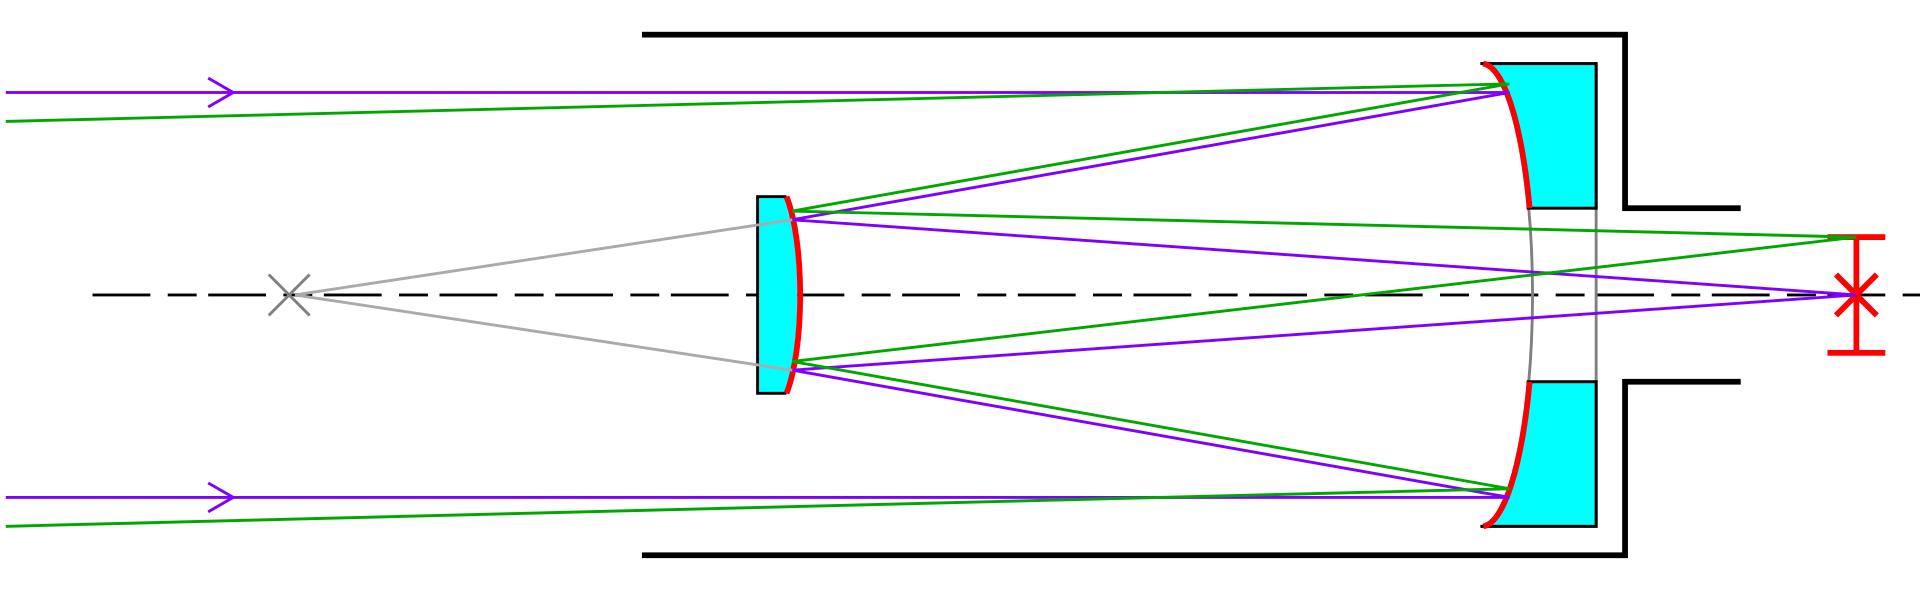
\includegraphics[width=0.6\linewidth]{lens.png}
	\caption{Schematic light path in a Cassegrain telescope\cite{manual}.}%
	\label{Fig:telescope}	
\end{figure}

% The spatial resolution is given by the Rayleigh criterion,
% \begin{eqnarray}
% \Delta\theta = 1.22 \frac{\lambda}{\text{D}}
% \end{eqnarray}
% \noindent
% where, \text{D} is the primary aperture and $ \lambda $ is the wavelength of light rays. The actual resolution is always very less for ground based telescope due to the numerous effect of Earth's atmosphere. \\
%
\subsubsection{Seeing and Airmass}
The earth's atmosphere has considered as a part of the optical system for ground based astronomical observation. So, numerous effect are arises, mostly, turbulence in the atmosphere leads fluctuation on refractive index on short spatial and temporal scale. This result in a blurring and scintillation of the PSF. That complicated shape can be represented by approximately Gaussian shape in two dimensions. Thus, the full width at half maximum(FWHM) size of the Gaussian shape of such stellar image is called Seeing of the image. It helps to measure the actual resolution in a particular observation. For Bonn, a seeing is 2 arcsec is a best value.\\

The column density on the atmosphere through which the light travels compared to vertical in-fall is called Airmass. For an angular distance z from zenith the best approximation can be computed as,
\begin{equation}
	a=\frac{1}{cos z}
\end{equation}
Where, $ a=1 $ for an object at the zenith i.e. $ z= 0^{\circ} $ and $ a=\infty $ at horizon.
Thus, the best possible observing position is near the zenith.\\

\subsubsection{Magnitude}
In optical astronomy, the optical brightness of a source is called magnitude.

The difference in magnitudes between two sources is defined on the basis of ratio of their observed fluxes $ \text{S}_{1} $ and $ \text{S}_{2} $ as,
\begin{equation}
	\Delta \text{m}= \text{m}_{1}-\text{m}_{2}=-(100^{1/5}). \log_{10} \bigg(\frac{\text{S}_{1}}{\text{S}_{2}}\bigg)
\end{equation}
From definition it is clear the fainter sources have higher magnitude.\\

\subsubsection{Coordinate system}
There are different co-ordinate systems (like as equatorial co-ordinate system, galactic co-ordinate system, and etc.) use to quantify the position of celestial objects in optical astronomy. Here, equatorial system is a most common system for identifying and cataloging the sources. In this system the framework of terrestrial latitude and longitude projected from the centre of earth onto the sky.
\begin{itemize}
	\item Declaration is an analogy to latitude in geography. Here, the north pole having declination of $ \delta=90^{\circ} $ and projection of south pole is  $ \delta= -90^{\circ} $. It is express as degree, minute and second. 
	\item Right Ascension, $\alpha $, is equivalent to longitude with the equatorial zero point. It is express as hour, minute and second.
\end{itemize}

\subsection{CCD Characteristics}
CCDs are the composition of essentially pure silicon based two-dimensional pixel detector, so it response wide wavelength range (from near infrared to the soft X-ray). The physical  light deflection mechanism involved in a CCD is the photoelectric effect. They have 2D array of light sensitive pixels having size, typically,  10 $ \mu $ to 20 $ \mu $. \\ 

The distribution of photons is converted to a distribution of charge packets which are collected and stored in three dimensional potential wells. To measure the amount of charge in each packets they have to be transported across the full detector surface to output amplifier. During this transportation of charge packets potential barriers in the transport direction can be manipulated by applying appropriate voltage waveform. The transport is done by parallel shift and series shift. On this functioning principle electrons are shifted, detected and converted in a digital number or count or analog-to-digit unit (ADU) at a rate of about 30 kHz. \\ 

The best CCDs have high quantum efficiency, low read noise, and excellent linearity. In this experiment we will determine these properties. Some of these properties are discussed below:

\subsubsection{Quantum Efficiency}
Quantum efficiency is define as The ratio of produced electrons to the number of photons hitting the detector surface. It is determine by the photon absorbing capacity of silicon in given wavelength. The best CCDs have high quantum efficiency, low read noise, and excellent linearity. In this experiment we will determine these properties.Top order CCDs have the significant wavelength range more than 90$\% $.

\subsubsection{Read-Out Noise}
An empty CCD, read out have a small scatter in signal level from pixel-to-pixel due to the amplification noise occurring in the electronics. The standard deviation of this scatter is called read out noise. The main sources of amplification noise are size of amplifier, integrated circuit contraction and temperature of amplifier.

\subsubsection{Stability}
There are several aspect to hold excellent stability characteristic by a CCD. Some of them are:
\begin{itemize}
	\item  CCD is geometrically very stable because it is contracted by pure silicon.
	\item It keeps its performance over years without degradation.
	\item It has very high sensitivity; however, very insensitive to over-exposure.
\end{itemize}

\subsubsection{Dark Current}
The dark current is a thermal noise which is composed of electrons liberated by thermal energy. It is depend on temperature of CCD. At room temperature  it fills CCD pixels to their saturation level within a short period of time (a minute or even less).Therefore, it is necessary to keeps the detector system at a low temperature. The cooing of CCD is done thermo-electrically with closed cycle system or by using liquid nitrogen. It is a less advantageous property of CCDs.\\

The dark current, $ \text{I}_{\text{dark}} $ ( measured in the unit of $ e^{-}/\text{Pix/\text{S}} $. ) increases exponentially with temperature, T, as
\begin{equation}
 \text{I}_{\text{dark}}=c. \text{T}^{3/2}.e^{-{\frac{\text{E}_{\text{g}}}{2k_{\text{B}}\text{T}}}}
 \label{Equ:DarkCurrent}
\end{equation}
Where, $ \text{E}_{\text{g}}= 1.16 $ eV is the silicon band gap energy, $ k_{\text{B}}=8.62 . 10^{-5} $ eV/K is the Boltzmann constant, and $ c $ is a detector specific constant.

\subsubsection{Gain}
The ratio, k, between the amount of charge in a CCD pixel and the corresponding digital number after A/D conversion is called detector gain. It is measured in the unit of $ e^{-}/ADU $. It can be derived based on the assumption that photons( or electrons) numbers are explained by Poison statistics. i.e. in a detector area with constant flat illumination the variance $ \sigma^2_{e} $ of the pixel to pixel fluctuation equal to the average number of electrons per pixel $\text{N}_{e} $. 
\begin{equation}
\text{N}_{e}= \sigma^2_{e}= k\text{N}_{e, \text{d}}= k^2 {\sigma}^2_{e,\text{d}}
\end{equation}
Where, $\text{N}_{e, \text{d}}$ and $ \sigma_{e,\text{d}} $ are the corresponding numbers after A/D conversion.Therefore, to calculate the gain we have to determine the average signal level and variance in a well exposed area of the detector and using following expression,
\begin{equation}
k=\frac{\text{N}_{e, \text{d}}}{\sigma^2_{e,\text{d}}}
\end{equation} 

\subsubsection{Noise}
Noise always means that the standard deviation of the signal level. In ou detector system there are two other noise components in the data which have to be separated. First one is read out noise (RON) and second is pixel-to-pixel fluctuation noise due to different quantum efficiency of different pixels. This is so-called Pixel Response Non-Uniformity (PRNU) noise. Thus, the total noise is given by,
\begin{equation}
\sigma_{\text{tot}}=\sqrt{ \sigma^2_{\text{RON}} + \sigma^2_{e} + \sigma^2_\text{PRNU}}
\end{equation}
Where, $ \sigma_{\text{PRNU}} $ gives small deviation in QE from pixel-to-pixel and it is also directly proportional to $ \text{N}_{e} $ given by,
\begin{equation}
\sigma_{\text{PRNU}}=\text{N}_{e} \text{f}_{\text{PRNU}}
\end{equation} 
Where, $ \text{f}_{\text{PRNU}} $ is the detector dependent characteristic PRNU factor. It is typically in the order of 0.01.

\subsubsection{Linearity and full-well capacity}
One the most appealing feature of CCDs as astronomical detectors is their linearity. Here, the output signal is proportional to the incoming photons received by the detector. They are linear over the full dynamic range of $10^4 $ to $10^5 $ and deviation from linearity is just $\pm 0.5 \%$  for well behaved system.\\
 
 The CCD pixels have limited charge capacity. The maximum number of the electrons fitting into a single pixel is called full well capacity. It can measure in the unit of $ e^{-} $. The  scientific CCDs have $ 100000 e^{-} $ full well capacity. If the pixels get full well then the CCD shows blooming effect. Saturation level is the range of a CCD signal, so it is measure in the unit of ADU.  
